\documentclass{beamer}

\usetheme[progressbar=frametitle]{metropolis}
\usepackage{appendixnumberbeamer}
\usepackage{amsmath}
\usepackage{bbold}

\usepackage{dsfont}
\usepackage{booktabs}
\usepackage[scale=2]{ccicons}
\usepackage{textpos}
\usepackage{xcolor,colortbl}
\usepackage{pgfplots}
\usepgfplotslibrary{dateplot}
\usepackage{url}
\usepackage[utf8]{inputenc}
\usepackage[T1]{fontenc}
\usepackage{tikzstyles}
\usepackage{textcomp}
\usepackage{pgfplots}
\usepackage{ulem}
\pgfplotsset{compat=1.14}
\usepackage{subfigure} 
\usepackage{mathabx}
\usepackage{hyperref}


\usepackage[
	backend=biber,
	citestyle=authoryear,
	bibstyle=authoryear,
	maxnames=2]{biblatex}
	\bibliography{bibliography.bib}

\usepackage{caption}
\captionsetup{font=scriptsize,labelfont=scriptsize}

% Math symbols
\newcommand{\E}{\mathbb{E}}
\newcommand{\Var}{\mathrm{Var}}
\newcommand{\Cov}{\mathrm{Cov}}

\newcommand\independent{\protect\mathpalette{\protect\independenT}{\perp}}
\def\independenT#1#2{\mathrel{\rlap{$#1#2$}\mkern2mu{#1#2}}}
\DeclareMathOperator*{\argmax}{arg\,max}

\tikzset{
  block/.style    = {draw, thick, rectangle, minimum height = 3em, minimum width = 3em},
  causalvar/.style      = {draw, circle, node distance = 2cm}
}

% Criteo colors/template (legacy)
\definecolor{criteoOrange}{RGB}{248,152,29}

% New names
\definecolor{cOrange}{RGB}{248,152,29}
\definecolor{cBlue}{RGB}{43,46,173}
\definecolor{cGreen}{RGB}{20,171,103}
\definecolor{cRed}{RGB}{248,88,29}

\setbeamercolor{structure}{fg=cOrange,bg=white}
\usepackage{helvet}
\setbeamertemplate{blocks}[rounded]

% https://www.overleaf.com/latex/templates/metropolis-beamer-theme/qzyvdhrntfmr
\addtobeamertemplate{frametitle}{}{%
\textblockcolour{white}
\begin{textblock*}{100mm}(.825\textwidth,-1.08cm)%.825\textwidth,,-1cm)
\includegraphics[scale=.205]{CAIL_logo}%0.3
\end{textblock*}}

\setbeamerfont{normal text}{size=\small}

\title{Interpretability and Adversarial Attacks}
\author{Ugo Tanielian}

\begin{document}

\begin{frame} 	 
\titlepage
\end{frame}

\begin{frame}[fragile]{Outline}
  \tableofcontents
\end{frame}

\section{Motivation}

\begin{frame}{Deep Learning for Images: A sucess story ?}

\begin{itemize}
    \item In the last decade, Deep Learning has achieved great successes in computer vision
    
    \begin{figure}[H]
        \centering
        \includegraphics[width=0.8\linewidth]{images/image_net_perf.png}
    \end{figure}
    
    \item What does it mean to below the human bias ?
    \item Are we chasing the right metric ?
    \item Does it mean we can really trust these models in real environments ? when human safety is at stake ? (e.g. self-driving cars)
\end{itemize}
\end{frame}

\begin{frame}{Accuracy vs Robustness ?}
    \begin{figure}[H]
    \centering
    \includegraphics[width=0.8\linewidth]{images/pig_attack.png}
    \end{figure}
    
    \begin{figure}[H]
    \centering
    \includegraphics[width=0.6\linewidth]{images/stop_sign.png}
    \end{figure}
\end{frame}

\begin{frame}{A generalization / data issue ?}
    More generally, the assumption that train and test distribution are the same is wrong in general
    \begin{figure}
    \centering
    \includegraphics[width=0.6\linewidth]{images/distribution_mismatch.png}
    \end{figure}
\end{frame}

\begin{frame}{Calibration \& Robustness}
    \begin{itemize}
        \item Can we trust neural networks ?
        \item Modern neural networks, unlike those from a decade ago, are poorly calibrated \cite{guo2017calibration}.
        \item Inputs that are unrobust are more likely to have poorly calibrated predictions \cite{qin2021improving}.
        \item Temperature scaling is the simplest, fastest way to remedy the miscalibration phenomenon in neural networks.
    \end{itemize}
\end{frame}

\begin{frame}{Calibration \& Robustness: \cite{guo2017calibration}}
    \begin{figure}
        \centering
        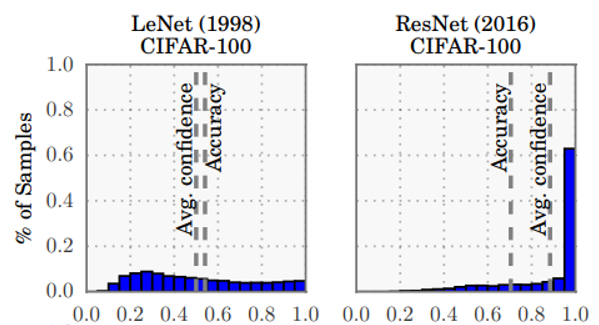
\includegraphics[width=0.65\linewidth]{images/calibration1.PNG}
    \end{figure}
    
    \begin{figure}
        \centering
        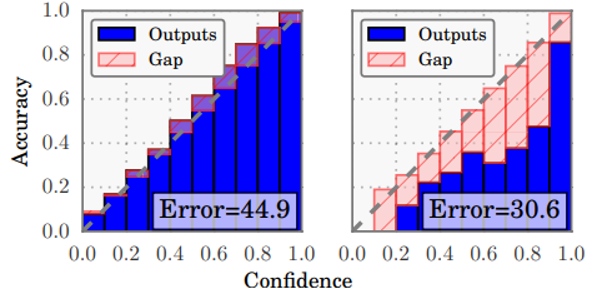
\includegraphics[width=0.6\linewidth]{images/calibration2.PNG}
    \end{figure}
\end{frame}


\begin{frame}{Even one pixel attacks can work}
    \begin{itemize}
        \item The results show that $67.97\%$ of the natural images in Kaggle CIFAR-10 test dataset and $16.04\%$ of the ImageNet (ILSVRC 2012) test images can be perturbed to at least one target class.
    \end{itemize}
    \begin{figure}
    \centering
    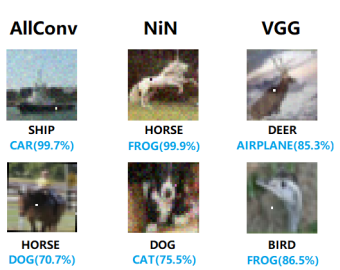
\includegraphics[width=0.6\linewidth]{images/one_pixel_attack.PNG}
    \caption{\cite{su2019one}}
    \end{figure}
\end{frame}

% \section{Interpretation}
% \begin{frame}{Maps}
% \end{frame}

\section{Attacks}

\begin{frame}{Attack onthology}
    \begin{itemize}
        
        \item Poisoning Attack: Contamination during the training phase
        \begin{itemize}
            \item Data Injection
            \item Data Modification
            \item Logic Corruption
        \end{itemize}
        
        \vspace{0.5cm}
        \item Evasion Attack: Malicious samples during testing phase. 
        \begin{itemize}
            \item White Box
            \item Black Box
        \end{itemize}
        
        \vspace{0.5cm}
        \item Exploratory Attack: Gaining knowledge about the algorithm
        \vspace{-0.5cm}
        \begin{itemize}
            \item Model inversion
            \item Model extraction
            \item Inference Attack (data P training set ?)
        \end{itemize}
    \end{itemize}
\end{frame}

\begin{frame}{Poisoning attacks}
    It is an attack type that takes advantage of your ML model \textbf{during training (as opposed to evasion attacks).}
    \begin{itemize}
        \item The goal is to corrupt the training set so that generalization is impacted.
        \item Poisoning attacks come in two flavors — those targeting your availability or integrity (“backdoor” attacks).
        \item Backdoor attacks are much more sophisticated. They leave your classifier functioning exactly like it should — with just one exception: a backdoor. A backdoor is a type of input that the model’s designer is not aware of, but that the attacker can leverage \cite{chen2017targeted}. 
    \end{itemize}
\end{frame}

\begin{frame}{Poisoning attacks}
    \begin{figure}
    \centering
    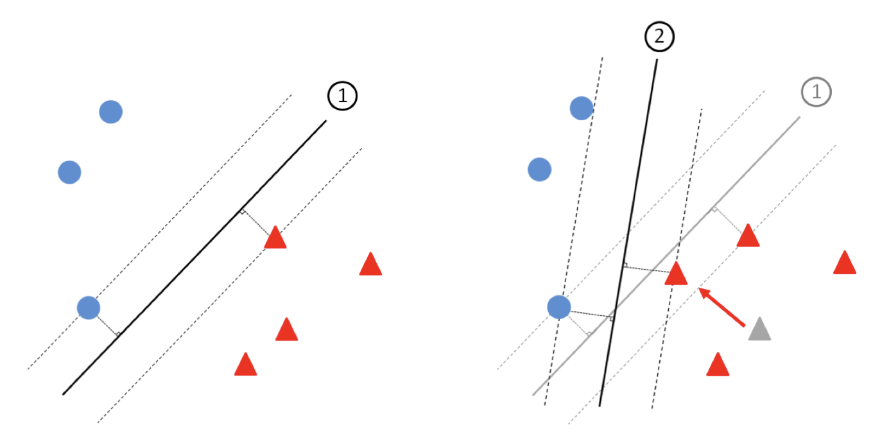
\includegraphics[width=0.90\linewidth]{images/data_poisoning_1.png}
    \caption{Decision boundary is significantly impacted in this example if just one training sample is changed, even when that sample’s class label does not change (right):\cite{miller2020adversarial}}
    \end{figure}
\end{frame}

\begin{frame}{Poisoning attacks (2)}
    \begin{figure}
    \centering
    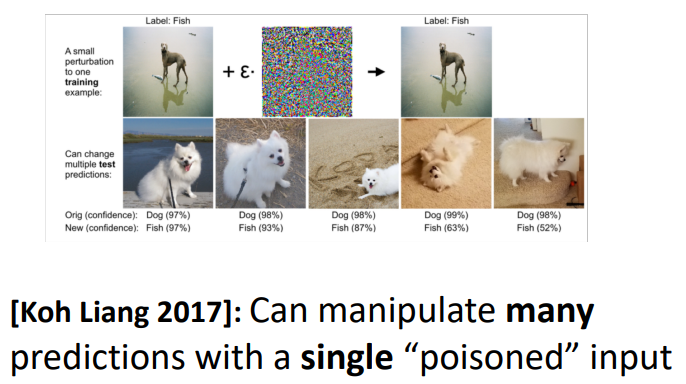
\includegraphics[width=1.\linewidth]{images/data_poisoning_3.png}
    %\caption{Decision boundary is significantly impacted in this example if just one training sample is changed, even when that sample’s class label does not change (right):\cite{miller2020adversarial}}
    \end{figure}
\end{frame}

\begin{frame}{Poisoning defenses}
    \begin{itemize}
        \item The most common type of defenses is \textbf{outlier detection}, also knows as \textit{“data sanitization” and “anomaly detection”}. 
        \item Sometimes the poison injected is indeed from a different data distribution and can be easily isolated.
    \end{itemize}
    \begin{figure}
    \centering
    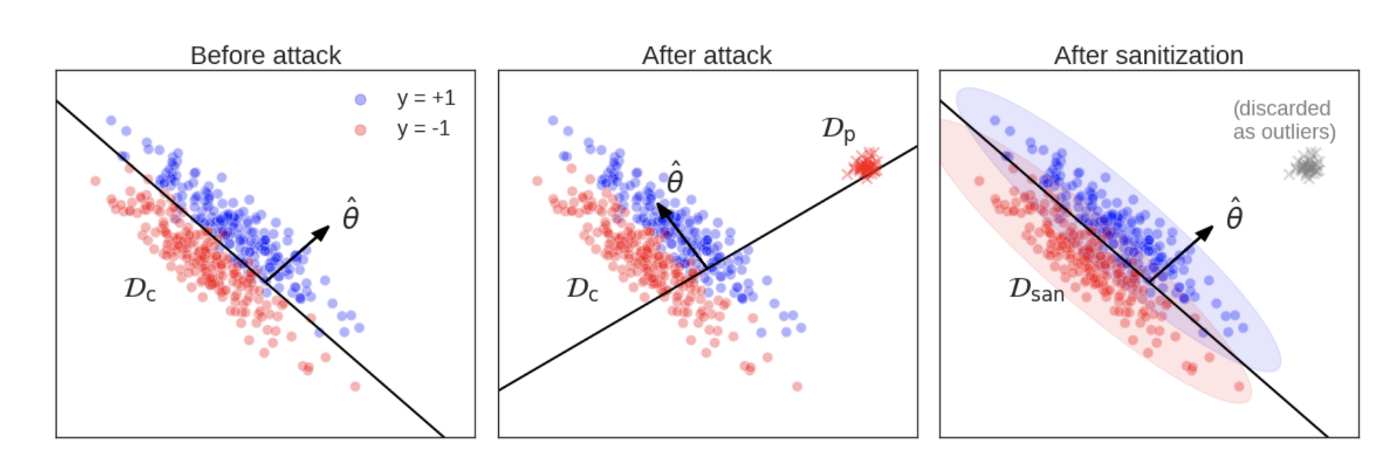
\includegraphics[width=0.9\linewidth]{images/data_poisoning_2.png}
    \caption{y discarding outliers from $D = D_c \bigcup D_p$: \cite{koh2021stronger}}
    \end{figure}
\end{frame}

\begin{frame}{Evasion attacks}
    An \textbf{evasion attack} happens when the network is fed an “adversarial example” — a carefully perturbed input that looks and feels exactly the same as its untampered copy to a human — but that completely throws off the classifier.
    
    \textbf{All models can be attacked !}
    \begin{itemize}
        \item Video: \href{https://github.com/advboxes/AdvBox/blob/master/applications/StealthTshirt/README.md}{Adversarial boxes}
        \item Audio: \href{https://nicholas.carlini.com/code/audio_adversarial_examples/}{Audio adversiarial examples}
    \end{itemize}
\end{frame}

\begin{frame}{Why a model can be attacked ?}
    \begin{enumerate}
        \item \textit{Szegedy}: the presence of low-probability “pockets” in the manifold (ie too much non-linearity) and poor regularization of networks.
        \item \textit{Goodfellow}: too much linearity in modern machine learning and especially deep learning systems
        \item \textit{The tilted boundary}: networks do not fit data perfectly (or lack training samples): there are adversarial pockets of inputs that exist between the boundary of the classifier and the sub-manifold of sampled data. (+ criticism of 1 and 2)
        \item \textit{Adversarial Examples Are Not Bugs, They Are Features}: humans are limited to 3 dimensions and can’t distinguish noise patterns from one another. Networks are a pattern recognition machine more sophisticated than ourselves.
        \item Link with High frequencies ?
    \end{enumerate}
\end{frame}

\begin{frame}{Evasion attacks}
    \begin{itemize}
        \item Happens at inference time.
        \item Usually find small perturbation on an input such that the confidence or the prediction changes.
        \item Black box (the attacker to know anything about the model) vs White box (requires access to the model).
    \end{itemize}
    \textbf{\begin{figure}[H]
        \centering
        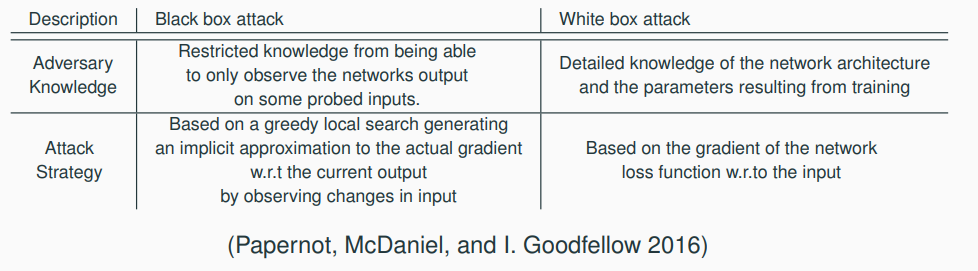
\includegraphics[width=0.85\linewidth]{images/black_vs_white_box.PNG}
        \caption{Adversarial attacks: Towards Deep Learning Models Resistant to Adversarial Attacks (2017).}
    \end{figure}}
\end{frame}

\begin{frame}{What is an adversarial attack ?}
    \begin{figure}[H]
        \centering
        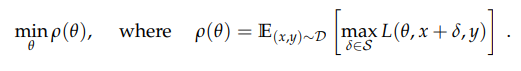
\includegraphics[width=1.0\linewidth]{images/adversarial_robustness.PNG}
        \caption{Adversarial attacks: Towards Deep Learning Models Resistant to Adversarial Attacks (2017).}
    \end{figure}
    \textbf{It is a worst-case mindset/scenario.}
\end{frame}

\begin{frame}{SOTA Attacks}
    \begin{enumerate}
        \item FGSM
        \item BIM
        \item Iterative Least Likely Method
        \item DeepFool
        \item CW (\cite{carlini2017towards})
    \end{enumerate}
\end{frame}

\begin{frame}{FGSM (Fast Gradient Sign Method)}
\begin{itemize}
    \item Introduced in I. J. Goodfellow et al. 2014.
    \item Main idea: compute the sign of the gradient $\nabla$ of the loss wrt to each pixel of the input image.
    \item Move in the opposite direction of $\nabla$ by a step of size $\varepsilon$.
    \item FGSM increases the cost function with the correct label, hoping that this will be enough to change the prediction.
    \item We obtain a perturbation of size $\varepsilon$ in $\|.\|_\infty$.
\end{itemize}
    \begin{figure}[H]
        \centering
        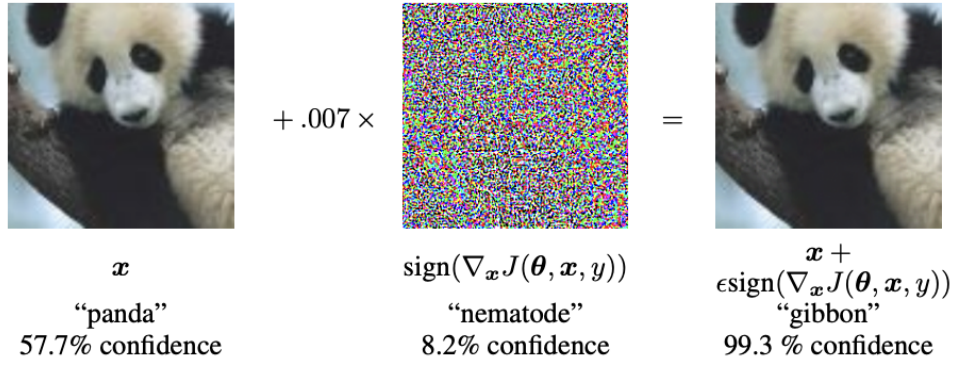
\includegraphics[width=0.75\linewidth]{images/FGSM.PNG}
        \caption{FGSM: Explaining and Harnessing Adversarial Examples (2014).}
    \end{figure}
\end{frame}

\begin{frame}{BIM (Basic Iterative Method) }
    \textbf{Main idea:} Apply FGSM several times while ensuring that we stay in an $\varepsilon$-ball around the original image w.r.t. the $\|.\|_\infty$ norm.
        \begin{figure}[H]
        \centering
        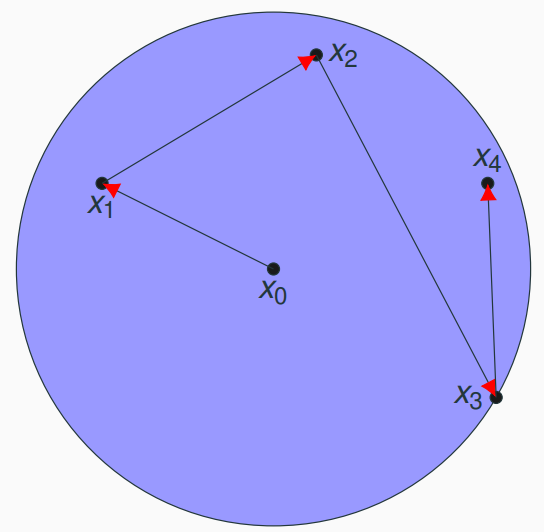
\includegraphics[width=0.5\linewidth]{images/BIM.PNG}
        %\caption{DeepFool for a linear, binary classifier. From Moosavi-Dezfooli et al. DeepFool: A Simple and Accurate Method to Fool Deep Neural Networks (2016).}
    \end{figure}
\end{frame}

\begin{frame}{Iterative Least Likely Method}
\begin{itemize}
    \item Both of the previous methods are untargeted attacks.
    \item By changing the BIM algorithm to alter the image towards a specific target class, it yields the Iterative Gradient Sign Method.
    \item Now, we target the Least Likely class, to give an idea on the worst case scenario.
\end{itemize}
\end{frame}

\begin{frame}{DeepFool}
    \begin{itemize}
        \item The DeepFool algorithm searches for an adversary with the smallest possible perturbation. 
        \item The algorithm tries to shift the image towards the closest decision boundary. 
    \end{itemize}
    \begin{figure}[H]
        \centering
        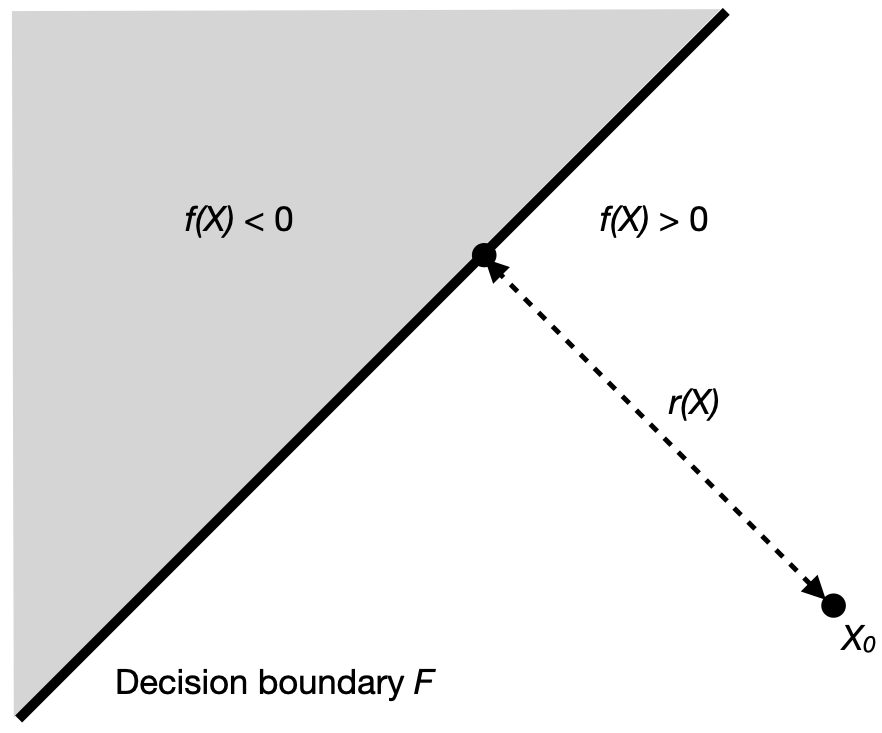
\includegraphics[width=0.5\linewidth]{images/DeepFool.png}
        \caption{DeepFool for a linear, binary classifier. From Moosavi-Dezfooli et al. DeepFool: A Simple and Accurate Method to Fool Deep Neural Networks (2016).}
    \end{figure}
\end{frame}

\begin{frame}{Some examples}
    \href{https://www.neuralception.com/adversarialexamples-attacks}{\textbf{NeuroCeption}}
\end{frame}

\section{SOTA Defenses}

\begin{frame}{Data augmentation with adversarial examples}
    \begin{itemize}
        \item A simple but yet effective way to defend against attacks is to add attacked images to the training set.
        \item It is attack specific: cumbersome process.
        \item Findings: FGSM adversaries don’t increase robustness (for large $\varepsilon$): that the network overfits to these adversarial examples. 
    \end{itemize}
    
    \textbf{Other theoretical questions}
    \begin{itemize}
    \item Standard image distribution lay on low dimension manifold (the manifold hypothesis) \cite{fefferman2016testing}.
        \item Sample complexity of adv. robust generalization can be significantly larger than that of “standard” generalization.
        \item Adversarially Robust Generalization Requires More Data \cite{schmidt2018adversarially}.
    \end{itemize}
\end{frame}

\begin{frame}{Defensive distillation}
\begin{itemize}
    \item Another solution proposed in \cite{papernot2016distillation} is based on \textbf{knowledge distillation}. 
    \item Main idea is to transfer knowledge from a teacher model to a student model (Hinton et al. 2015).
\end{itemize}
\begin{figure}
        \centering
        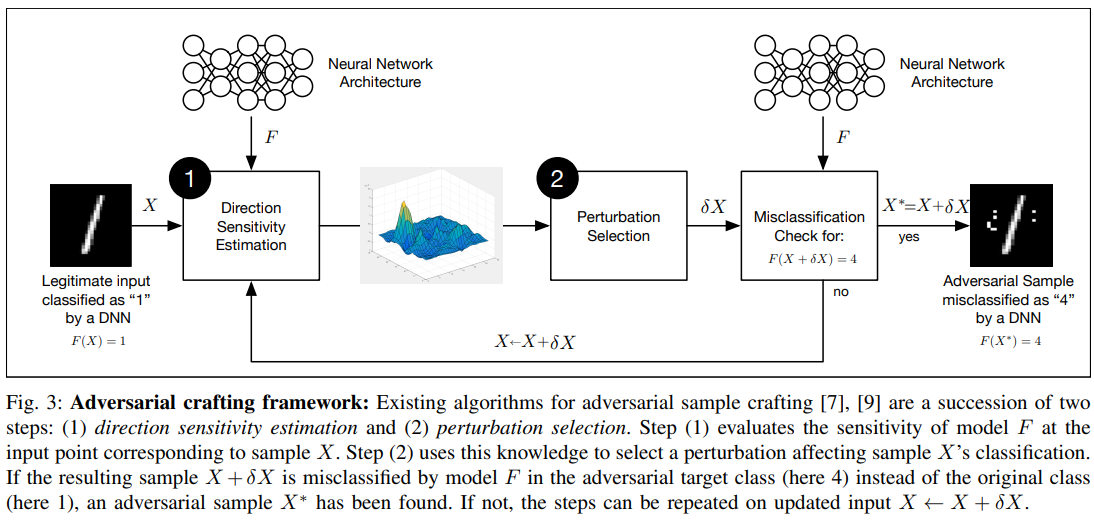
\includegraphics[width=1.0\linewidth]{images/distillation_framework.PNG}
        %\caption{DeepFool for a linear, binary classifier. From Moosavi-Dezfooli et al. DeepFool: A Simple and Accurate Method to Fool Deep Neural Networks (2016).}
    \end{figure}
\end{frame}

\begin{frame}{Gradient penalty}
    There is a connection between robustness and regularizing the gradient of the network \cite{bietti2018regularization}.
    
    How can we implement this regularization ? 
    \begin{itemize}
        \item Clipping
        \item A gradient penalty
        \item Spectral normalization
    \end{itemize}
    
\end{frame}

\begin{frame}{Label smoothing}
    \begin{figure}
    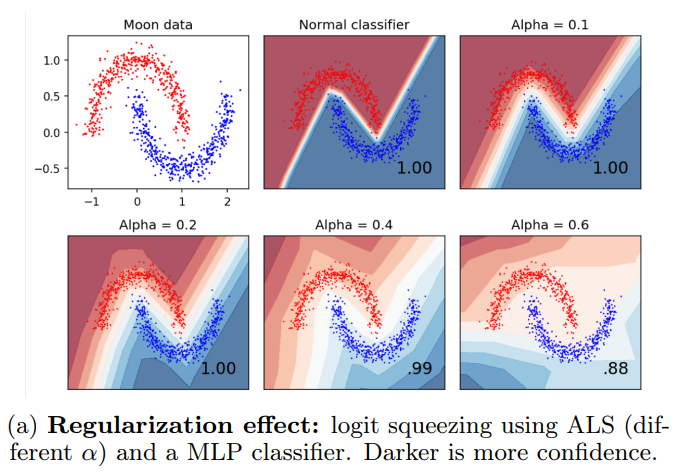
\includegraphics[width=0.90\textwidth]{images/adversarial_label_smoothing.PNG}
    \caption{Regularization effect of LS \cite{goibert2019adversarial}.}
    \end{figure}

\end{frame}

\begin{frame}{Last but not least: Distributional robustness}
    \begin{itemize}
        \item We know that many problem arise from doing pure \textbf{Empirical Risk Minimization}.
        \item One way to circumvent this limitation is to treat the empirical distribution $\mu_n$ with skepticism and to replace it with an uncertainty set $\mathcal{U}(\mu_n)$ of distributions around $\mu_n$.
        \item This gives rise to the distributionally robust obejctive \cite{blanchet2019data, blanchet2019robust}:
        %\item Note that it is a function of $\theta$, $\varepsilon$ and the class of divergence/distance chosen.
    \end{itemize}
\end{frame}

\begin{frame}{DRO}
    \begin{figure}
    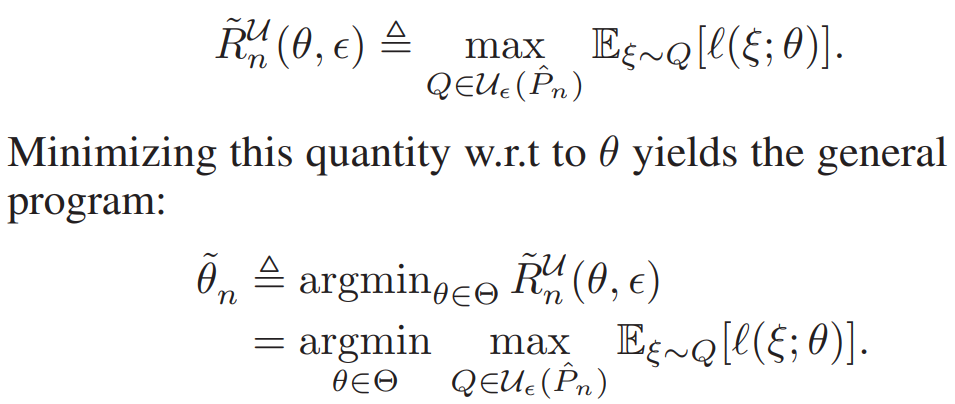
\includegraphics[width=0.90\textwidth]{images/dro_objective.PNG}
    \end{figure}
    There is liberty on the way to construct $U_\varepsilon(\hat{P}_n)$.
    \begin{figure}
    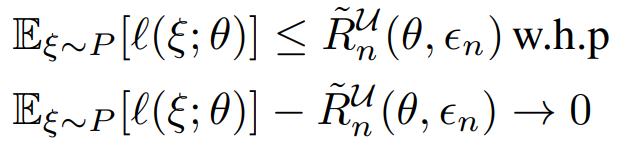
\includegraphics[width=0.6\textwidth]{images/dro_guarantees.PNG}
    \end{figure}
\end{frame}

\begin{frame}{GANs for robustness}
    \begin{figure}
    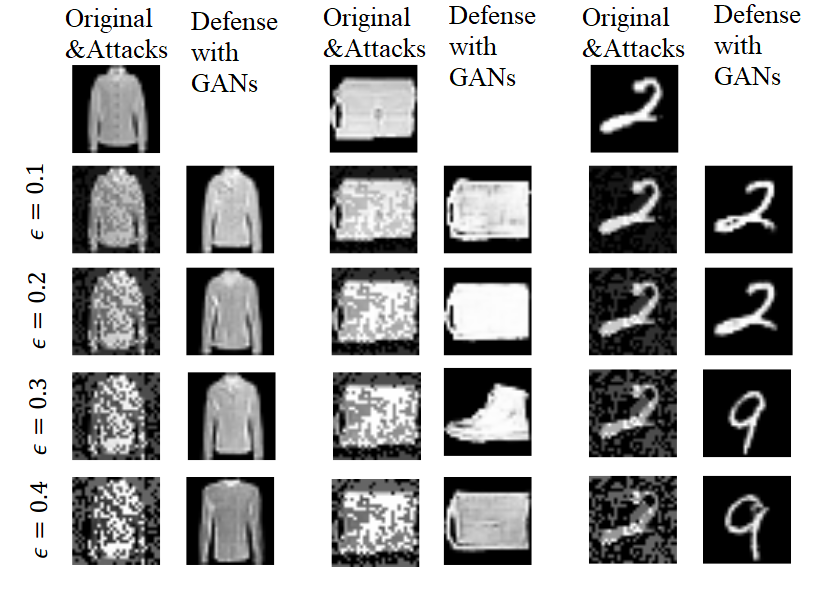
\includegraphics[width=0.80\textwidth]{images/defenseGANs.png}
    \caption{Defending deep nets with GANs: \cite{samangouei2018defense}.}
    \end{figure}
\end{frame}

% \section{Detections}
% \begin{frame}{SOTA Detection}
% \begin{itemize}
%     \item LID (\cite{ma2018characterizing})
%     \item Mahalanobis (\cite{lee2018simple})
% \end{itemize}
% \end{frame}

\section{Beyond adversarial robustness}
\begin{frame}{Robustness \& accuracy}
    \begin{itemize}
        \item Can we get both robustness and accuracy ?
        \item We could think that a robust model will also generalize better. 
        \item Counter-example found by \cite{tsipras2018robustness}, where the authors exhibit a dataset where you cannot be both accurate and robust at the same time.
        \begin{theorem}
            On the above dataset, any classifier that attains at least $1-\delta$ standard accuracy has robust accuracy at most $\frac{p\delta}{a-p}$ against an $\|.\|_\infty$-bounded adversary.
        \end{theorem}
        
    \end{itemize}
\end{frame}

\begin{frame}{No free lunch theorem ?}

\begin{itemize}
    \item Understanding the tradeoff between accuracy and
robustness is a very active line of research. 
    \item See for instance the strong "no free lunch" theorem from \cite{dohmatob2018limitations} "on a very broad class of data distributions, any classifier with even a bit of accuracy is vulnerable to adversarial attacks".
\end{itemize}
\end{frame}

\section{Just for fun}
\begin{frame}{Generating images with robust network}
    \begin{figure}
    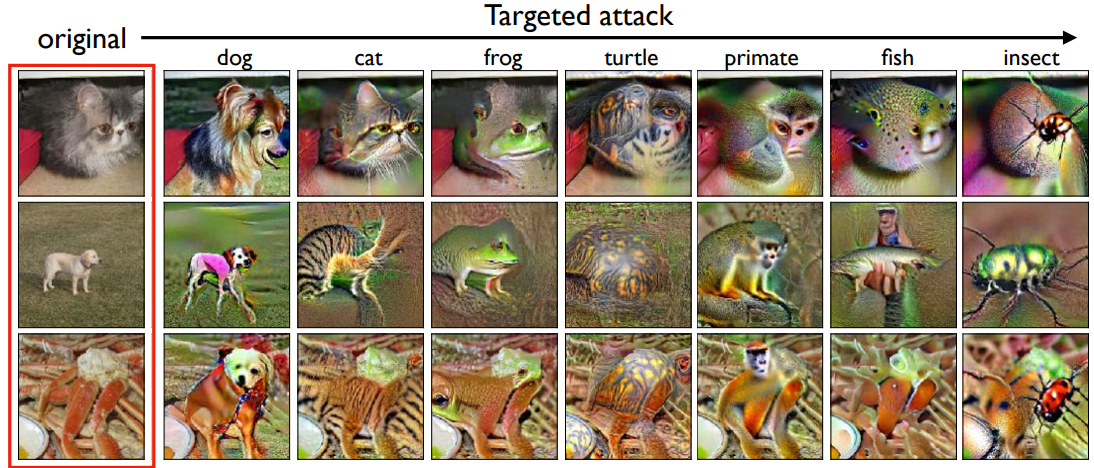
\includegraphics[width=1.\textwidth]{images/robust_classifier_targeted_attack.PNG}
    \caption{\cite{santurkar2019image}}
    \end{figure}
\end{frame}

\begin{frame}{Generating images with robust network (2)}
    \begin{figure}
    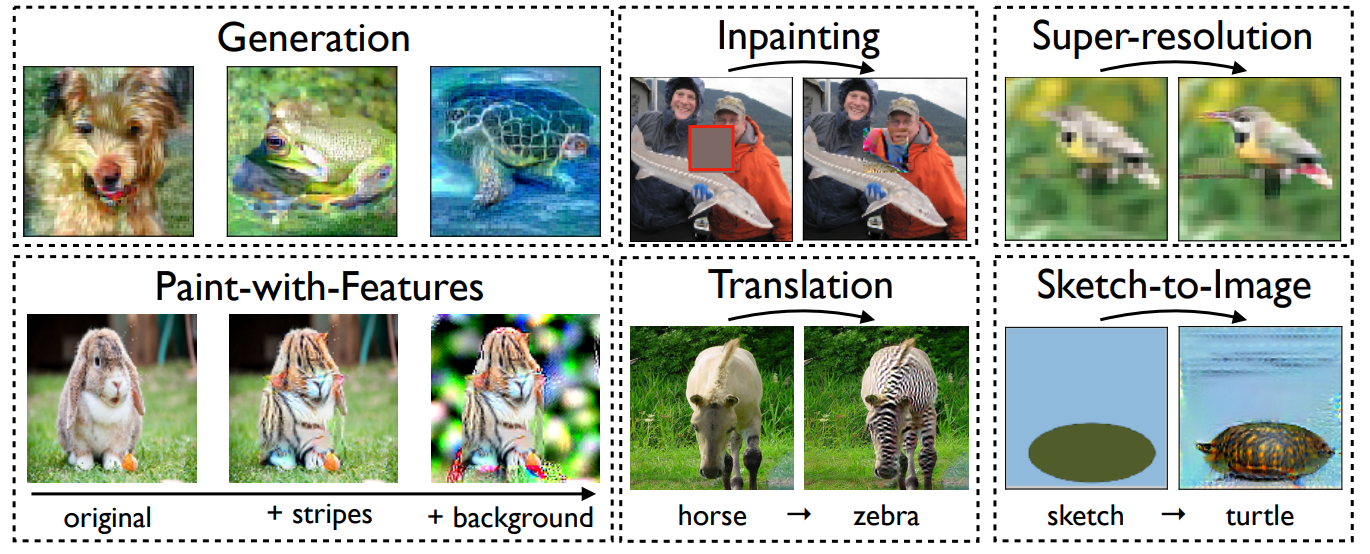
\includegraphics[width=1.\textwidth]{images/generation_with_robust_classifier.PNG}
    \caption{\cite{santurkar2019image}}
    \end{figure}
\end{frame}

\section{Interesting information}
\begin{frame}{Robustness from the Madry lab}
\href{https://github.com/MadryLab/robustness}{Robustness package:}
one can
\begin{itemize}
    \item Train and evaluate standard and robust models on a variety of datasets/architectures.
    \item Import pre-trained robust models.
\end{itemize}
\end{frame}

\begin{frame}{Adversarial Robustness Toolbox}
    \begin{itemize}
        \item \href{https://github.com/Trusted-AI/adversarial-robustness-toolbox}{Adversarial Robustness Toolbox (ART)} is a Python library for Machine Learning Security.
        \item ART provides tools that enable developers and researchers to evaluate, defend, certify and verify Machine Learning models and applications against the adversarial threats of Evasion, Poisoning, Extraction, and Inference.
    \end{itemize}
\end{frame}

\begin{frame}{A survey on robustness}
\begin{figure}
    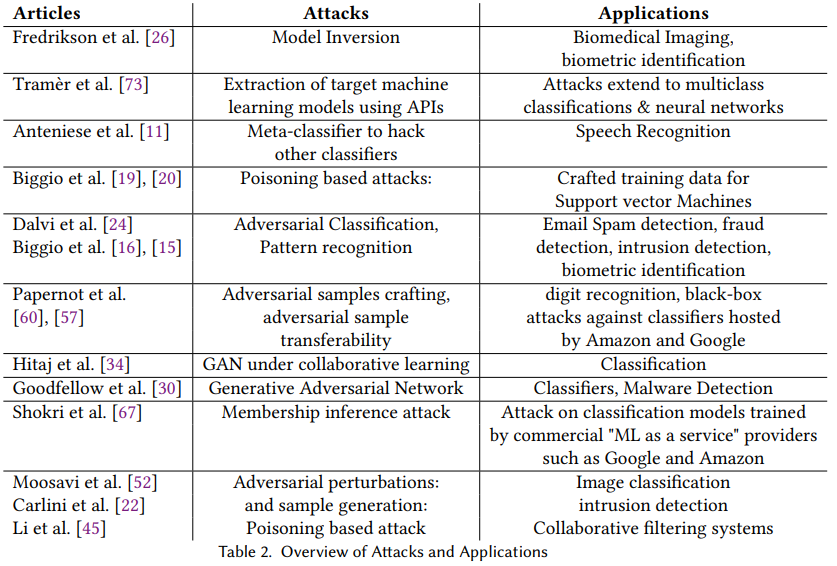
\includegraphics[width=1.\textwidth]{images/robustness_survey.PNG}
    \caption{\cite{chakraborty2018adversarial}}
    \end{figure}
\end{frame}

\begin{frame}{Conclusion}
    \textbf{Three commandments of Secure/Safe ML}
    \begin{enumerate}
        \item You shall not train on data you don’t fully trust
(because of data poisoning). 
\item You shall not let anyone use your model (or observe its
outputs) unless you completely trust them (because of model stealing and black box attacks). 
\item You shall not fully trust the predictions of your model
(because of adversarial examples)
    \end{enumerate}
\end{frame}

\section*{References}
\begin{frame}[allowframebreaks]\small
  \frametitle{References}
  \renewcommand*{\bibfont}{\footnotesize}
  \printbibliography
\end{frame}

\end{document}
